\documentclass{scrartcl}
\usepackage{mm_ws15}
\usepackage{mathabx}
\usetikzlibrary{quotes,angles,arrows,decorations.markings}


\newcommand{\xx}{\vec x}
\newcommand{\yy}{\vec y}
\newcommand{\zz}{\vec z}

\newcommand{\uu}{\mat u}
\newcommand{\vv}{\mat v}
\newcommand{\ww}{\mat w}


\newcommand{\sheetTitle}{Blatt 3, Abgabe 10.11.2015 12:00} 
\begin{document}
\maketitle

\section{Direkte Beweise}
Beweisen Sie die folgenden Aussagen. 
Übersetzen Sie außerdem Aussagen, die ausformuliert sind, in formale mathematische Aussagen und umgekehrt.
\begin{subex}
  \item Für alle reellen Zahlen $x$, die größer als 1 sind, ist $6x + 3$ größer als $3x + 6$.
  \item Das Quadrat aller geraden natürlichen Zahlen ist wieder gerade.
  \item Alice ist 16 Jahre alt. Damit ist Alice genau doppelt so alt, wie Bob war, als Alice so alt war, wie es Bob jetzt ist. Bob ist 12 Jahre alt.
  \item $\forall k, m \in \NN\colon k + m \le k \times m \implies k \ge 2 \land m \ge 2$
  \item $\forall p, q \in \RR\colon (\forall x \in \RR\colon x^2 + px + q > 0) \iff \left( \frac{p^2}{2} < q \right)$ 
\end{subex}

\begin{remark}{Hinweise}
  Für b) benutzen Sie die folgende Definition: $n \in \NN$ heißt gerade, wenn es ein $n' \in \NN$ gibt, sodass $n = 2n'$. 
  \quotes{$\land$} steht für das logische UND.
  \todo{More remarks! Example? What is $\implies$, what is $\iff$}
\end{remark}

\begin{solution}[Beispiel]
  Beweisen Sie, dass die Summe zweier gerader Zahlen wieder gerade ist.\\

  \emph{Formal:} $\forall m, n \in \NN; m, n \mbox{ gerade} \implies (m + n) \mbox{ gerade}.$

  \emph{Beweis:} Da $m$ und $n$ gerade sind existieren lt.\ Definition $m', n' \in \NN$, sodass $m = 2m'$ und $n = 2n'$. Damit folgt, dass $m + n$ gerade ist, da
  \[
    m + n = 2m' + 2n' = 2 (m' + n').
  \] 

  Den selben Beweis kann man mit weniger Prosa wie folgt aufschreiben:
  \begin{align*}
    m, n \mbox{ gerade} 
    &\iff \exists m', n' \in \NN\colon m = 2m' \land n = 2n' \\
    &\implies m + n = 2 (m' + n') \\
    &\implies (m + n) \mbox{ gerade}
  \end{align*}
\end{solution}


\section{Euklidisches Skalarprodukt}
In der Vorlesung wurde das euklidische Skalarpodukt in $\RR^n$ definiert durch
\[
  \sp{\cdot}{\cdot} \colon \RR^n \times \RR^n \to \RR, (\uu, \vv) \mapsto \sp{\uu}{\vv} = \sum_{k=1}^n u_k v_k.
\]
\begin{subex}
  \item Zeigen Sie, dass $\sp{\cdot}{\cdot}$ ein Skalarprodukt auf $\RR^n$ ist, d.h.\ die drei Eigenschaften eines Skalarprodukts erfüllt sind (siehe unten).
  \item Berechnen Sie $\sp{\uu}{\vv}$, $\norm{\uu}$ und $\norm{\vv}$ für 
  \[
    \uu = \colvec{1 \\ 0 \\ 3} \quad\mbox{und}\quad \colvec{-5 \\ 2 \\ 1}.
  \]
  Hier bezeichnet $\norm{\uu} = \sqrt{\sp{\uu}{\uu}}$ die induzierte Norm.
  \item Finden Sie alle Vektoren $\vv \in \RR^2$, die mit $\uu = \colvec{1 \\ 2}$ das Skalarprodukt $\sp{\uu}{\vv} = 2$ haben.  
  \item Welche der folgenden Beispiele definiert ein Skalarprodukt auf $V$?
  Überprüfen Sie jeweils die Bedingungen an ein Skalarprodukt.
  \begin{itemize}
    \item $V = \RR^3, \sp{\uu}{\vv} = 2u_1 v_1 +u_2 v_2 +5u_3 v_3$
    \item $V = \RR^2, \sp{\uu}{\vv} = u_2 v_2 + u_1 v_1$
    \item $V =\RR^2 \sp{\uu}{\vv} = 2u_1 v_1 + u_1 v_2 + u_2 v_1 + 3u_2 v_2$
    \item $V =\RR^2 \sp{\uu}{\vv} = 2u_1 v_1 + u_1 v_2 + 3u_2 v_1 + u_2 v_2$
  \end{itemize}
\end{subex}


\section{Skalarprodukt\,\&\,Winkel}
Der Kosinussatz, welcher Ihnen vielleicht aus der Schule bekannt ist, stellt eine Beziehung in einem Dreieck zwischen den Seiten $a,b,c$ und dem der Seite $c$ gegenüberliegendem Winkel $\varphi$ her.
Er lautet
  \[
  c^2=a^2+b^2-2ab\cos \varphi.
  \]
\begin{subex}
  \item Leiten Sie diese Beziehung her, dabei soll Ihnen die Skizze als Inspiration dienen.
  \item Benutzen Sie den Kosinussatz um für beliebiges $n \in \NN$ folgendes zu zeigen: Für $\uu, \vv \in \RR^n$ gilt:
  \[
    \cos \sphericalangle(\uu,\vv) = \frac{\sp{\uu}{\vv}}{\norm{\uu}\,\norm{\vv}}
  \] 
  Hierbei bezeichnet $\sphericalangle(\uu,\vv)$ den von $\uu$ und $\vv$ aufgespannten Winkel.
\end{subex}

\begin{center}
  \begin{tikzpicture}[
    scale=1,
    baseline/.style={line width=1pt}
  ]

  \coordinate (A) at (5,0);
  \coordinate (B) at (0,0);
  \coordinate (C) at (2,2);

  \draw (A) -- (B) node[midway, below] {$a$};
  \draw (B) -- (C) node[midway, above left] {$b$};
  \draw[dotted] (C) -- (A) node[midway, above right] {$c$};

  \draw pic["$\varphi$",draw,angle eccentricity=0.6,angle radius=1cm,line width=.5pt] {angle=A--B--C};
  
  \end{tikzpicture}
\end{center}


\section{Das Methanmolekül}
Ein Methanmolekül (chemische Formel $\mathrm{CH}_4$) besitzt die Struktur eines regulären Tetraheders (siehe Bild).
Die Wasserstoffatome (weiß) befinden sich dabei in den Punkten $(0,0,0)$, $(k,k,0)$, $(k,0,k)$ und $(0,k,k)$; das Kohlenstoff im Zentrum im Punkt $(\frac{k}{2},\frac{k}{2},\frac{k}{2})$.
Hierbei bezeichnet $k$ eine Längenkonstante.
\begin{subex}
  \item Zeigen Sie, dass die angegebene Struktur tatsächlich einen regulären Tetraheder bilden, d.h.\ dass alle Verbingslinien zwischen den Wasserstoffatomen gleich lang sind.
  \item Berechnen Sie den Bindungswinkel zwischen zwei Wasserstoffatomen, d.h.\ den Winkel, der von zwei Wasserstoffatomen mit dem Kohlenstoffatom im Scheitelpunkt aufgespannt wird.
\end{subex}

\begin{center}
  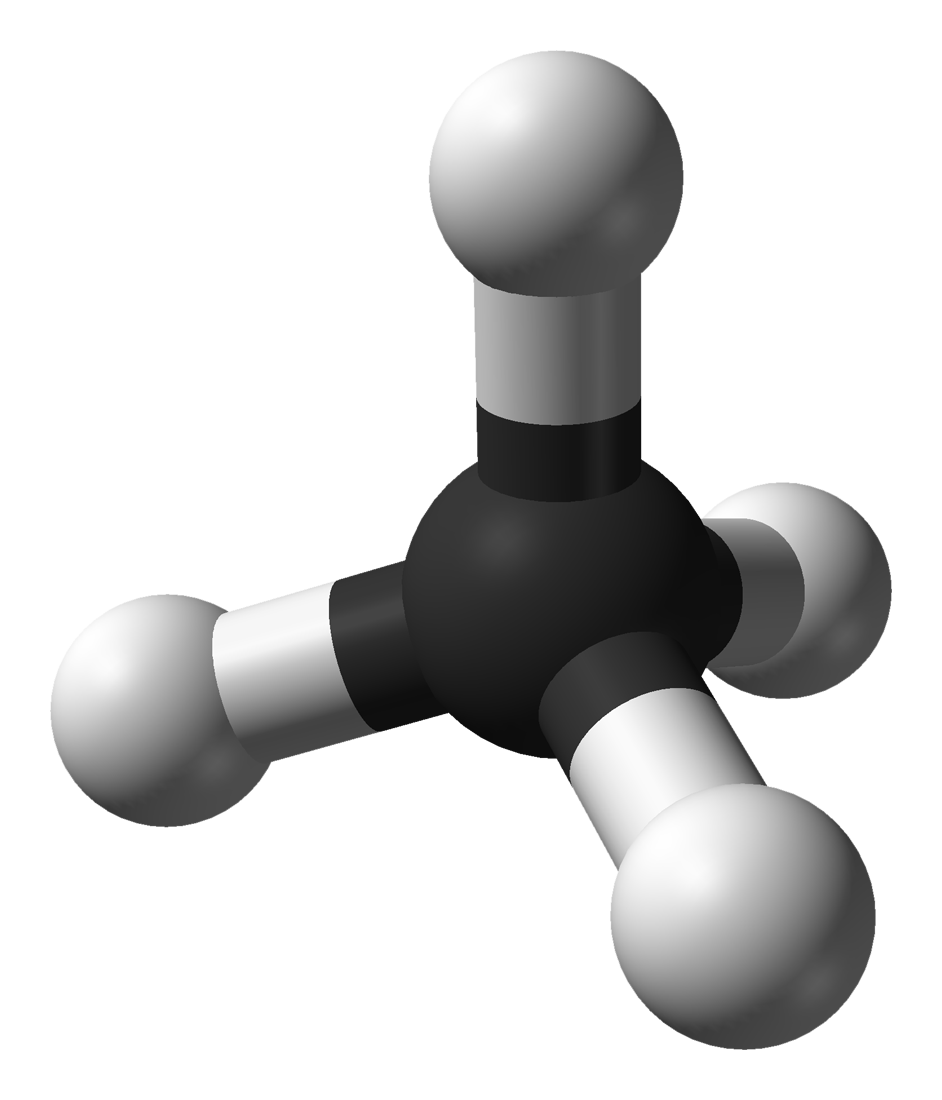
\includegraphics[width=3cm]{img/methan.png}
\end{center}


 

\end{document}
